% In your report, answer the following questions.
% A. Understand and analyze each calibration step from the camera calibration toolbox for Matlab
% B. Show the calibration results for the initialization and non-linear optimization steps
% C. Visualize the re-projection errors and extrinsic parameters (3D plot)

\section{Calibration steps}

% TODO: explain the concepts of focal lenght, principal point, distortion and
% pixel error

\section{Results}

After the initialization step of the calibration, we only have the
\textbf{focal length} and \textbf{principal point} intrinsic parameters. They
are presented in the table~\ref{tab:init_param}


\begin{table}[h]
  \centering
  \caption{Calibration parameters after initialization}\label{tab:init_param}
  \begin{tabular}{l N{5}{2} N{5}{2}}
    \toprule

    Focal length:       &   670.66552   &   670.66552   \\

    \midrule

    Principal point:    &   319.50000   &   239.50000   \\

    \bottomrule
  \end{tabular}
\end{table}

After the optimization we get more results; In addition to the recalculated focal lenght,
principal point, and their uncertainties, we get the camera \textbf{distortion}
and \textbf{pixel error} (and their uncertainties). The results can be found in
the table~\ref{tab:optim_param}

\begin{table}[h]
  \centering
  \caption{Calibration results after optimization (with uncertainties)}\label{tab:optim_param}
  \begin{tabular}{l N{5}{2} N{5}{2} N{5}{2} N{5}{2} N{5}{2}}
    \toprule

    Focal length:       &   662.21300   &   664.25919   \\
    +/-                 &   1.38569     &   1.50583     \\

    \midrule

    Principal point:    &   305.77235   &   243.22028   \\
    +/-                 &   2.68110     &   2.61929     \\

    \midrule

    Distortion:  &   -0.29040 &   0.36843 &   0.00032 &   0.00054 & 0.00000 \\
    +/-          &   0.01105  &   0.04833 &   0.00062 &   0.00064 & 0.00000 \\

    \midrule

    Pixel error:        &   0.51943 &   0.35333 \\

    \bottomrule
  \end{tabular}
\end{table}

The camera \textbf{skew} isn't calculated, because modern cameras are assumed
to have rectangular pixels. This is the default setting in the calibration
toolbox. Figure~\ref{fig:reprojection} has a visualization of the reprojection
error, and figure~\ref{fig:extrinsic} has the extrinsic parameters in a 3D plot.
% TODO:maybe explain the reprojection error and extrinsic parameters, or like,
% whats the point about visualizing them


\begin{figure}[h]
  \centering
  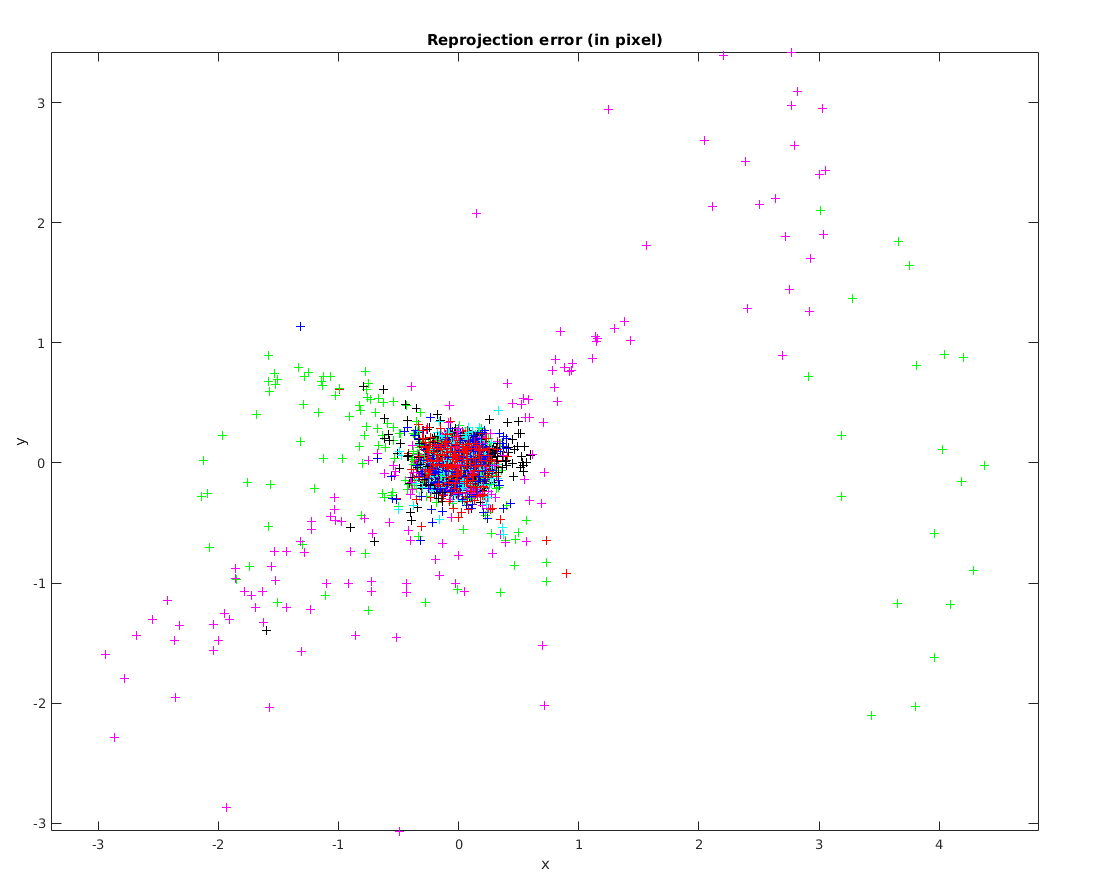
\includegraphics[width=0.8\linewidth]{reprojection_error}
  \caption{Visualization of the reprojection error}\label{fig:reprojection}
\end{figure}


\begin{figure}[h]
  \centering
  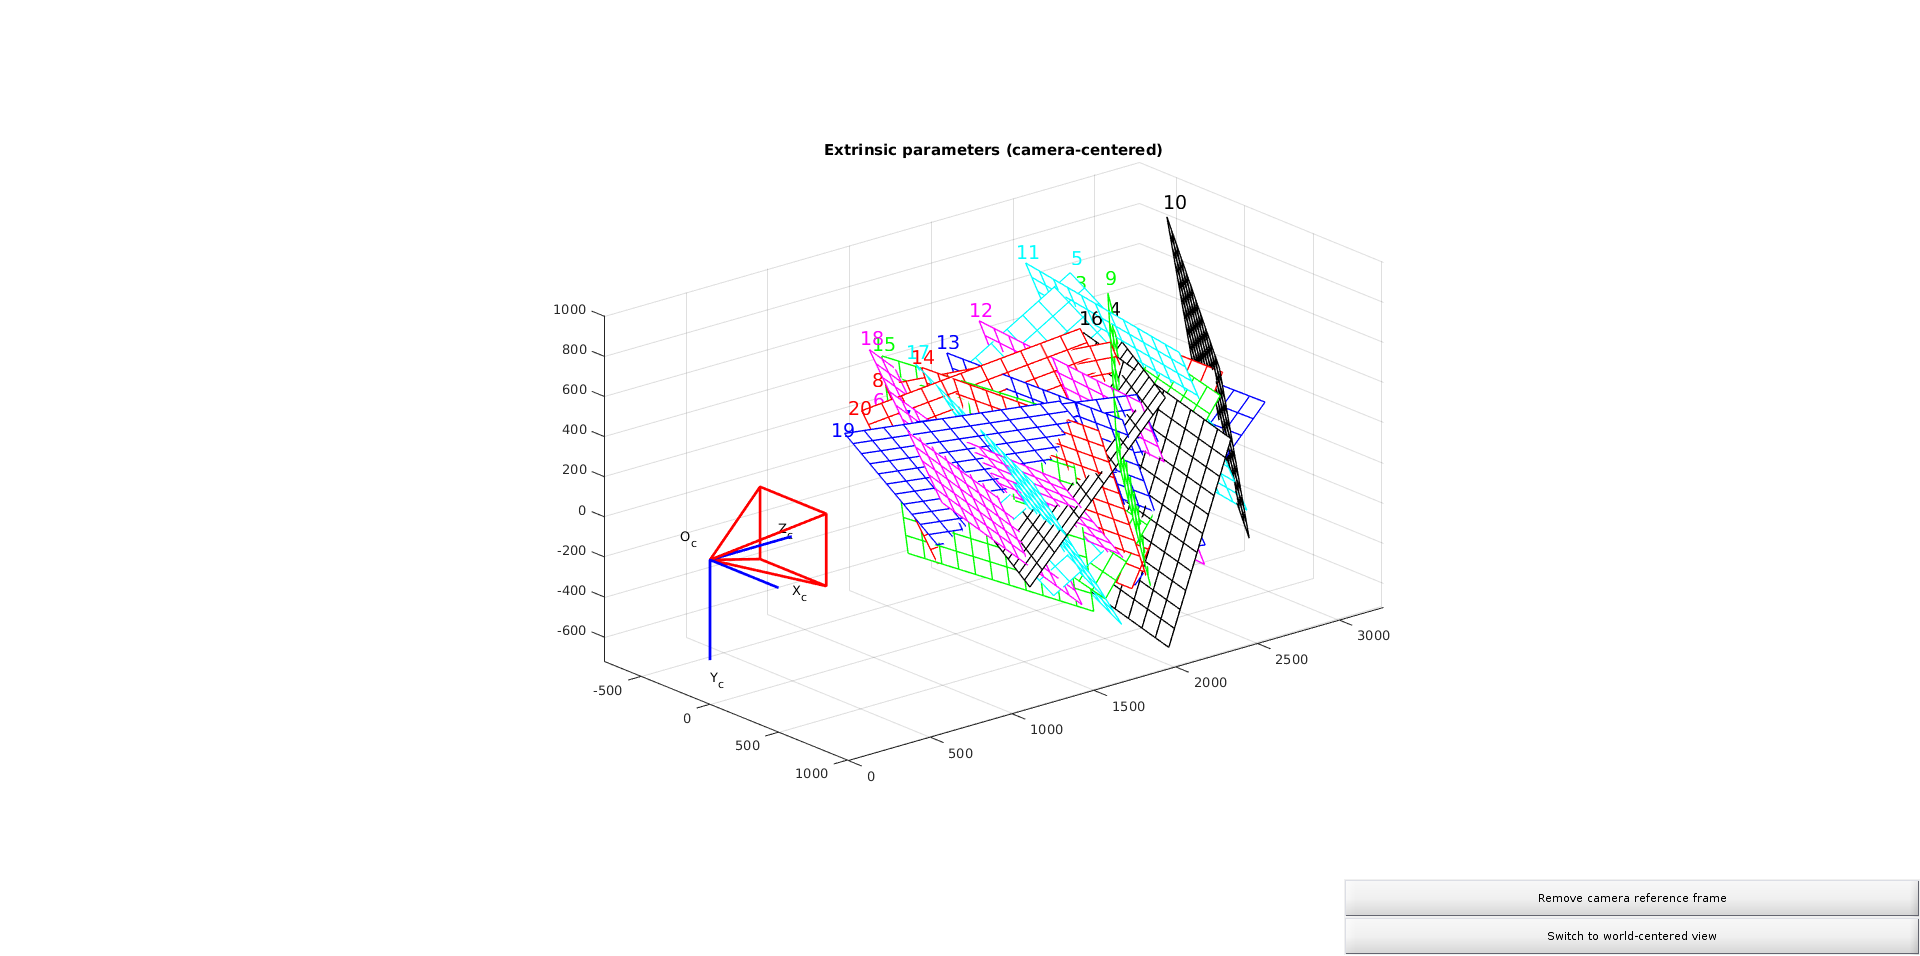
\includegraphics[width=0.8\linewidth]{extrinsic_cam_centered}
  \caption{Visualization of extrinsic parameters}\label{fig:extrinsic}
\end{figure}
